\documentclass[journal,12pt,twocolumn]{IEEEtran}

\usepackage{setspace}
\usepackage{gensymb}

\singlespacing


\usepackage[cmex10]{amsmath}

\usepackage{amsthm}

\usepackage{mathrsfs}
\usepackage{txfonts}
\usepackage{stfloats}
\usepackage{bm}
\usepackage{cite}
\usepackage{cases}
\usepackage{subfig}

\usepackage{longtable}
\usepackage{multirow}

\usepackage{enumitem}
\usepackage{mathtools}
\usepackage{steinmetz}
\usepackage{tikz}
\usepackage{circuitikz}
\usepackage{verbatim}
\usepackage{tfrupee}
\usepackage[breaklinks=true]{hyperref}

\usepackage{tkz-euclide}

\usetikzlibrary{calc,math}
\usepackage{listings}
    \usepackage{color}                                            %%
    \usepackage{array}                                            %%
    \usepackage{longtable}                                        %%
    \usepackage{calc}                                             %%
    \usepackage{multirow}                                         %%
    \usepackage{hhline}                                           %%
    \usepackage{ifthen}                                           %%
    \usepackage{lscape}     
\usepackage{multicol}
\usepackage{chngcntr}

\DeclareMathOperator*{\Res}{Res}

\renewcommand\thesection{\arabic{section}}
\renewcommand\thesubsection{\thesection.\arabic{subsection}}
\renewcommand\thesubsubsection{\thesubsection.\arabic{subsubsection}}

\renewcommand\thesectiondis{\arabic{section}}
\renewcommand\thesubsectiondis{\thesectiondis.\arabic{subsection}}
\renewcommand\thesubsubsectiondis{\thesubsectiondis.\arabic{subsubsection}}


\hyphenation{op-tical net-works semi-conduc-tor}
\def\inputGnumericTable{}                                 %%

\lstset{
%language=C,
frame=single, 
breaklines=true,
columns=fullflexible
}
\begin{document}


\newtheorem{theorem}{Theorem}[section]
\newtheorem{problem}{Problem}
\newtheorem{proposition}{Proposition}[section]
\newtheorem{lemma}{Lemma}[section]
\newtheorem{corollary}[theorem]{Corollary}
\newtheorem{example}{Example}[section]
\newtheorem{definition}[problem]{Definition}

\newcommand{\BEQA}{\begin{eqnarray}}
\newcommand{\EEQA}{\end{eqnarray}}
\newcommand{\define}{\stackrel{\triangle}{=}}
\bibliographystyle{IEEEtran}
\providecommand{\mbf}{\mathbf}
\providecommand{\pr}[1]{\ensuremath{\Pr\left(#1\right)}}
\providecommand{\qfunc}[1]{\ensuremath{Q\left(#1\right)}}
\providecommand{\sbrak}[1]{\ensuremath{{}\left[#1\right]}}
\providecommand{\lsbrak}[1]{\ensuremath{{}\left[#1\right.}}
\providecommand{\rsbrak}[1]{\ensuremath{{}\left.#1\right]}}
\providecommand{\brak}[1]{\ensuremath{\left(#1\right)}}
\providecommand{\lbrak}[1]{\ensuremath{\left(#1\right.}}
\providecommand{\rbrak}[1]{\ensuremath{\left.#1\right)}}
\providecommand{\cbrak}[1]{\ensuremath{\left\{#1\right\}}}
\providecommand{\lcbrak}[1]{\ensuremath{\left\{#1\right.}}
\providecommand{\rcbrak}[1]{\ensuremath{\left.#1\right\}}}
\theoremstyle{remark}
\newtheorem{rem}{Remark}
\newcommand{\sgn}{\mathop{\mathrm{sgn}}}
\providecommand{\abs}[1]{\left\vert#1\right\vert}
\providecommand{\res}[1]{\Res\displaylimits_{#1}} 
\providecommand{\norm}[1]{\left\lVert#1\right\rVert}
%\providecommand{\norm}[1]{\lVert#1\rVert}
\providecommand{\mtx}[1]{\mathbf{#1}}
\providecommand{\mean}[1]{E\left[ #1 \right]}
\providecommand{\fourier}{\overset{\mathcal{F}}{ \rightleftharpoons}}
%\providecommand{\hilbert}{\overset{\mathcal{H}}{ \rightleftharpoons}}
\providecommand{\system}{\overset{\mathcal{H}}{ \longleftrightarrow}}
	%\newcommand{\solution}[2]{\textbf{Solution:}{#1}}
\newcommand{\solution}{\noindent \textbf{Solution: }}
\newcommand{\cosec}{\,\text{cosec}\,}
\providecommand{\dec}[2]{\ensuremath{\overset{#1}{\underset{#2}{\gtrless}}}}
\newcommand{\myvec}[1]{\ensuremath{\begin{pmatrix}#1\end{pmatrix}}}
\newcommand{\mydet}[1]{\ensuremath{\begin{vmatrix}#1\end{vmatrix}}}
\numberwithin{equation}{subsection}
\makeatletter
\@addtoreset{figure}{problem}
\makeatother
\let\StandardTheFigure\thefigure
\let\vec\mathbf
\renewcommand{\thefigure}{\theproblem}
\def\putbox#1#2#3{\makebox[0in][l]{\makebox[#1][l]{}\raisebox{\baselineskip}[0in][0in]{\raisebox{#2}[0in][0in]{#3}}}}
     \def\rightbox#1{\makebox[0in][r]{#1}}
     \def\centbox#1{\makebox[0in]{#1}}
     \def\topbox#1{\raisebox{-\baselineskip}[0in][0in]{#1}}
     \def\midbox#1{\raisebox{-0.5\baselineskip}[0in][0in]{#1}}
\vspace{3cm}
\title{Assignment 1}
\author{Rubeena Aafreen (EE20RESCH11012)}
\maketitle
\newpage
\bigskip
\renewcommand{\thefigure}{\theenumi}
\renewcommand{\thetable}{\theenumi}
Download all python codes from 
\begin{lstlisting}
https://github.com/rubeenaafreen20/EE5609/tree/master/Codes
\end{lstlisting}
%
and latex codes from 
%
\begin{lstlisting}
https://github.com/rubeenaafreen20/EE5609
\end{lstlisting}
%
\section{Problem}
A ray of light passing through the point \myvec{1\\2}
reflects on the x-axis at point \vec{A} and the reflected ray passes through the point \myvec{5\\3}. Find
the coordinates of \vec{A}.
\section{Explanation}
Let point \vec{P} be \myvec{1\\2} and point \vec{Q} be \myvec{5\\3}
Since, point \vec{A} is on x-axis, its y-coordinate is zero.
Assume \begin{align}
    A=\myvec{k\\0}
\end{align}
Incident vector
 \begin{align}
     = \vec{P-A}
\end{align}
Reflected vector 
\begin{align}
    = \vec{Q-A}
\end{align}
Vector along y-axis
\begin{align}
\vec{e_1} =\myvec{1\\0}\\
\end{align}
Vector along x-axis
\begin{align}
 \vec{e_2} =\myvec{0\\1}
\end{align}

Angle between AP and the x axis = 180\degree - angle between AQ and the x axis,

\begin{align}
\dfrac{\vec{(P-A)^T} \Vec{e_2}}{\norm{\Vec{P-A}}}=\dfrac{\vec{(Q-A)^T} \Vec{e_2}}{\norm{\Vec{Q-A}}}
\\
\dfrac{\vec{P^T}\Vec{e_2}-\Vec{A^T}\Vec{e_2}}{ \norm{\Vec{P-A}}}=\dfrac{\vec{Q^T}\Vec{e_2}-\Vec{A^T}\Vec{e_2}}{\norm{\Vec{Q-A}}}
\end{align}

\section{Solution}
\begin{align}
 \dfrac{\myvec{1 & 2}\myvec{0\\1}-\myvec{k & 0}\myvec{0\\1}}{\norm{\myvec{1-k \\ 2}}}=\dfrac{\myvec{5 & 3}\myvec{0\\1}-\myvec{k & 0}\myvec{0\\1}}{\norm{\myvec{5-k\\3}}}
 \\
 \implies \dfrac{2}{\sqrt{(1-k)^2+(2)^2}}=\dfrac{3}{\sqrt{(5-k)^2+(3)^2}}
\end{align}
\begin{align}
    \label{eq:1}
       \implies 5k^2+22k-91=0 
\end{align}

Solving \eqref{eq:1} we get:
 k=2.6, -7 
 \\
 Since, incident ray passes through \myvec{1\\2} and reflected ray passes through \myvec{5\\3}},\\
 k cannot be negative as reflection takes place in first quadrant.
\begin{align}
   k=2.6
\end{align}
\section{Verification}
Figure plotted using python code:
\begin{figure}[h]
\centering
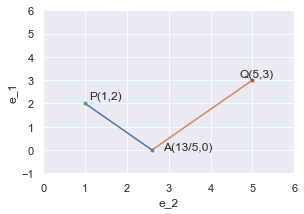
\includegraphics[width=\columnwidth]{output.png}
\caption{Incident and reflected ray vectors plotted via Python code}
\label{fig:1}
\end{figure}
\end{document}